\documentclass{layout/ost-report}

%% Set up the bibliography
\usepackage{biblatex}
\addbibresource{report.bib}

%% Additional packages and commands
\usepackage{parskip}
\setlist{itemsep=-2pt} % Reducing white space in lists slightly
\renewcommand{\deg}{\si{\degree}\xspace} % Use \deg easily, everywher

%% Custom Packages
\usepackage{tikz}
\usepackage{circuitikz}
\usepackage{subcaption}

%% ----------------------------------------------------------------------
%%    Begin of document + Frontmatter (Roman page numbering)
%% ----------------------------------------------------------------------

\begin{document}

\frontmatter

%% Define the main parameters
\title{A Title to the Report}
\subtitle{A Catchy Optional Subtitle \\ that Grabs the Attention}
\author{Fabio Zahner \& Silvan Lendi}

\subject{AiFo: AiFoundations} % Cover only

\affiliation{Ostschweizer Fachhochschule} % Cover only DE
%\affiliation{Eastern Switzerland University of Applied Sciences} % Cover only EN
%\affiliation{Haute École Spécialisée de Suisse Orientale} % Cover only FR
%\affiliation{Scuola Universitaria Professionale della Svizzera Orientale} % Cover only IT

\coverimage{figures/christmas-tree.jpeg} % Aspect ratio of 2:3 (portrait) recommended
\definecolor{title}{HTML}{D72964} % Color for cover title

\makecover

\begin{titlepage}

\begin{center}

%% Print the title
{\makeatletter
\largetitlestyle\fontsize{45}{45}\selectfont\@title
\makeatother}

%% Print the subtitle
{\makeatletter
\ifdefvoid{\@subtitle}{}{\bigskip\titlestyle\fontsize{20}{20}\selectfont\@subtitle}
\makeatother}

\bigskip
\bigskip

by

\bigskip
\bigskip

%% Print the name of the author
{\makeatletter
\largetitlestyle\fontsize{25}{25}\selectfont\@author 
\makeatother}

\bigskip
\bigskip

%% Print table with names and student numbers
\setlength\extrarowheight{2pt}
\begin{tabular}{lc}
    Silvan Lendi & 23-168-057\\\midrule
    Fabio Zahner & 23-167-315 \\
\end{tabular}

\vfill

%% Print some more information at the bottom
\begin{tabular}{ll}
    Instructor: & Lehmann Marco \\
    Submisstion Date: & 03.11.2024 \\
    Faculty: & Departement Informatik, Ostschweizer Fachhochschule OST \\
\end{tabular}

\bigskip
\bigskip

%% Add a source and description for the cover and optional attribution for the template
\begin{tabular}{p{15mm}p{10cm}}
    Cover: & https://www.pexels.com/photo/christmas-christmas-tree-gifts-tree-42294/ \\
    % Feel free to remove the following attribution, it is not required - still appreciated :-)
    Style: & OST Report Style, with modifications by Nico Fehr
\end{tabular}

%% Insert the OST logo at the bottom of the page
\begin{tikzpicture}
    \node[above=10mm] at (current page.south) {%
      
\includegraphics[width=0.35\linewidth]{layout/ost/ost-logo-de}
    };
\end{tikzpicture}

\end{center}

\end{titlepage}

\chapter*{Preface}
\addcontentsline{toc}{chapter}{Preface}

\emph{A preface...}

\begin{flushright}
{\makeatletter\itshape
    \@author \\
    OST, \monthname{} \the\year{}
\makeatother}
\end{flushright}

\chapter*{Summary}
\addcontentsline{toc}{chapter}{Summary}

\emph{A summary...}


\tableofcontents
%\listoffigures
%\listoftables

%\chapter*{Nomenclature}
\addcontentsline{toc}{chapter}{Nomenclature}

\emph{If a nomenclature is required, a simple template can be found below for convenience. Feel free to use, adapt or completely remove.}

\section*{Abbreviations}

\begin{longtable}{p{2.5cm}p{8cm}}
    \toprule
    Abbreviation & Definition \\
    \midrule\endhead % Add abbreviations alphabetically here:
    ISA & International Standard Atmosphere \\
    ... \\
    \bottomrule
\end{longtable}

\section*{Symbols}

\begin{longtable}{p{2.5cm}p{8cm}p{2.5cm}}
    \toprule
    Symbol & Definition & Unit \\
    \midrule\endhead % Add Latin symbols alphabetically here:
    $V$ & Velocity & [m/s] \\
    ... \\
    \midrule % Add Greek symbols alphabetically here:
    $\rho$ & Density & [kg/m$^3$] \\
    ... \\
    \bottomrule
\end{longtable}


%% ----------------------------------------------------------------------
%%    Mainmatter (Arabic page numbering)
%% ----------------------------------------------------------------------

\mainmatter

\chapter{Introduction}
\label{chapter:introduction}

This document details the implementation process for the AI Foundations module Miniproject. The project involves generating and evaluating at least three ideas that leverage a GPT-based assistant and building an application around the chosen concept.

The process begins with idea generation and selection based on defined evaluation criteria. Once an idea is selected, we refine it and develop specifications for the application.

Our goal was to choose an idea with practical utility—something we would personally use. During brainstorming, we considered common challenges where a large language model (LLM) could assist us. Within a short time, we generated three ideas:

\begin{itemize}
	\item A food recipe generator that provides recipes based on ingredients available at home (user input).
	\item A gift idea generator, inspired by the upcoming holiday season, which suggests gifts based on characteristics of the recipient.
	\item A belt balancer generator for the game \href{https://www.factorio.com}{Factorio}\footnote{Not affiliated with the product; however, we recommend trying it.}.
\end{itemize}

Next, we evaluated the practicality and feasibility of each idea. While all were potentially useful, the belt balancer idea presented significant complexity and implementation challenges. A belt balancer in Factorio helps distribute items across multiple input and output belts. Factorio allows players to import such structures as blueprint strings, which are encoded in base64 and compressed using zlib before translating into JSON for in-game structures.

Although it initially seemed promising, generating a valid belt balancer string with an LLM proved difficult. Even after ten attempts, none of the generated strings imported successfully into the game, so we decided to eliminate this idea.

We established the following criteria to evaluate the remaining ideas:

\begin{itemize}
	\item Practical use (weight: 30)
	\item Ease of implementation (weight: 5)
	\item Benefit (weight: 20)
	\item Originality (weight: 10)
\end{itemize}
\begin{table}[!h]
	\centering
	\renewcommand{\arraystretch}{1.3} % Increase row height for readability
	\begin{tabular}{|l|c|c|c|c|c|}
		\hline
		\textbf{Idea}       & \textbf{Practical Use} & \textbf{Ease of Implementation} & \textbf{Benefit}       & \textbf{Originality}   & \textbf{Total Score} \\
		\hline
		Recipe Generator    & $5 \times \mathbf{30}$ & $8 \times \mathbf{5}$           & $7 \times \mathbf{20}$ & $5 \times \mathbf{10}$ & \textbf{400}         \\
		\hline
		Gift Idea Generator & $7 \times \mathbf{30}$ & $8 \times \mathbf{5}$           & $9 \times \mathbf{20}$ & $8 \times \mathbf{10}$ & \textbf{510}         \\
		\hline
	\end{tabular}
	\caption{Evaluation of Project Ideas}
	\label{tab:project_idea_evaluation}
\end{table}

The Gift Idea Generator scored highest, so we selected it as our project.

Before implementation, we defined specifications for the application. We agreed on the following requirements:
The application should accept three input parameters: Gender, Age, and Personal Interests. It should also be accessible on mobile devices for convenient use on the go. When the user enters the parameters and presses the button to generate ideas, they should receive five gift suggestions in text form.


\chapter{About the Template}
%\label{chapter:title}

This template aims to simplify and improve the (Xe)LaTeX report/thesis template by OST with the following three main design principles:

\begin{itemize}
  \item \textbf{Simplicity First:} A class file that has been reduced by nearly 70\% to simplify customization;
  \item \textbf{Effortless:} A careful selection of common packages to get started immediately;
  \item \textbf{Complete:} Ready-to-go when it comes to the document and file structure.
\end{itemize}

\noindent This template works with pdfLaTeX, XeLaTeX and LuaLaTeX. In order to adhere to the OST house style, either XeLaTeX or LuaLaTeX is required, as it supports TrueType and OpenType fonts. BibLaTeX is used for the bibliography with as backend biber. Please visit \url{https://norukh.github.io/report/} for the full documentation.

\section*{Documentation (Abridged)}

As a report/thesis is generally a substantial document, the chapters and appendices have been separated into different files and folders for convenience. The folders are based on the three parts in the document: the frontmatter, mainmatter and appendix. All files are inserted in the main file, \texttt{report.tex}, using the \texttt{\textbackslash input\{filename\}} command. The document class, which can be found in \texttt{ost-report.cls}, is based on the book class. 

The template will automatically generate a cover when the \texttt{\textbackslash makecover} command is used. The title, subtitle and author will also be present on the title page. To give greater flexibility over the title page, the layout is specified in \texttt{title-report.tex}. A title page for theses is also available: \texttt{title-thesis.tex}. Change the corresponding \texttt{\textbackslash input\{...\}} command in the main file to switch. 

The bibliography has been set up in \texttt{report.tex} to allow for easy customization. It is included in the table of contents and renamed to 'References' using the \texttt{heading=bibintoc} and \texttt{title=References} options of the \texttt{\textbackslash printbibliography} command respectively. If you would like to use a different .bib file, change the command \texttt{\textbackslash addbibresource{report.bib}} accordingly.

\emph{→ Visit \url{https://norukh.github.io/report/} for the full documentation.}

\begin{figure}[h]
  \centering
  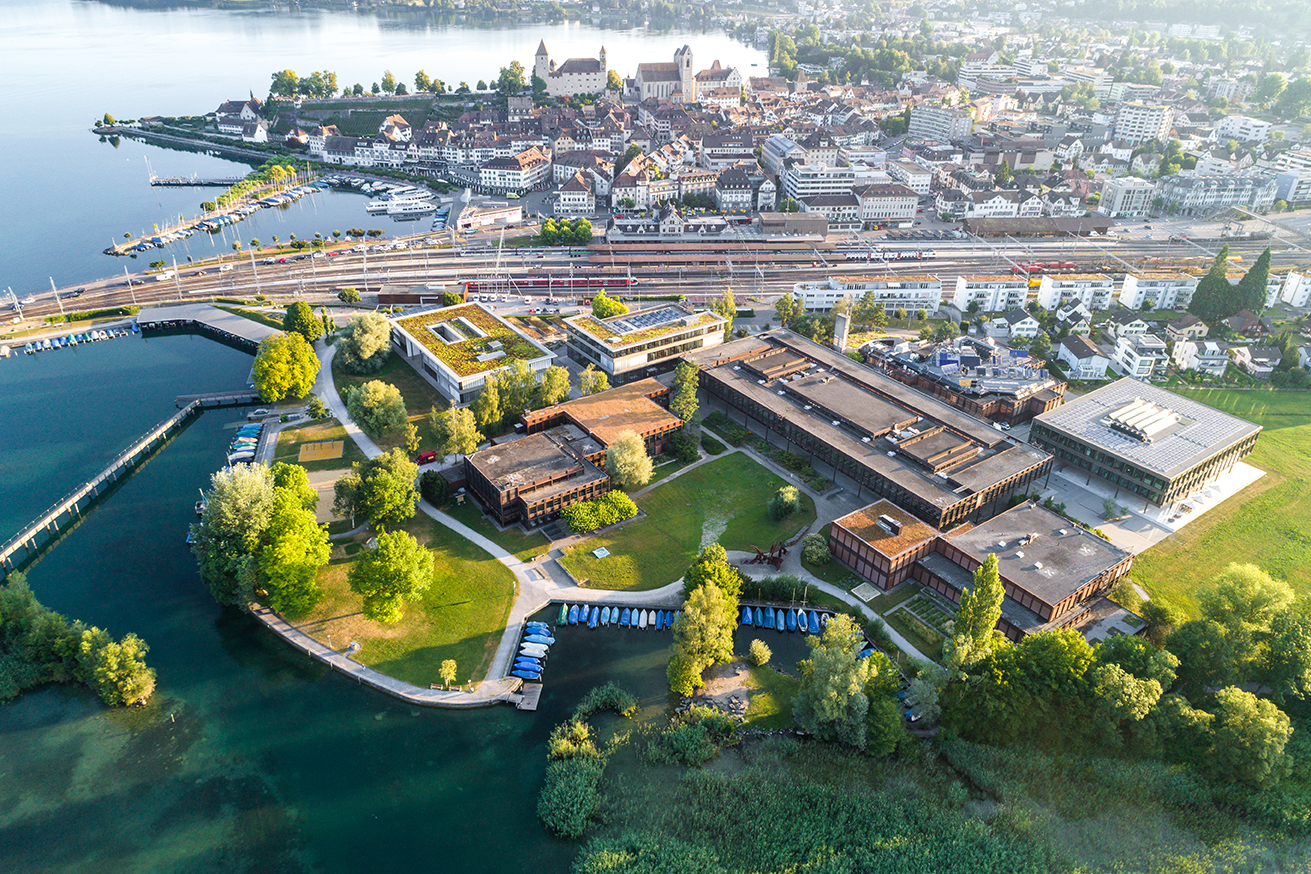
\includegraphics[width=0.95\linewidth]{figures/ost-campus-rj.jpg}
  \caption{OST Campus Rapperswil}
\end{figure}

\section*{License}

The origin of this template is the report/thesis template by Daan Zwaneveld, which is licensed under CC BY-NC 4.0.
This template has been adopted by Nico Fehr to the OST design and is licensed under CC BY-NC 4.0 as well. To view a copy of this license, visit \url{https://creativecommons.org/licenses/by-nc/4.0/}. No attribution is required in PDF outputs created using this template.
\chapter{Implementation: Frontend}
\label{chapter:implementation-frontend}

To create an application that integrates into daily life, we will use the Flutter technology stack to develop software accessible across multiple platforms. For development, we have focused on optimizing the application for Android mobile phones. However, if we decide to expand the application to other platforms, it would require minimal additional work.

\begin{figure}[!ht]
	\centering
	\resizebox{0.5\textwidth}{!}{%
		\begin{circuitikz}
			\tikzstyle{every node}=[font=\Large]
			\draw [ rounded corners = 19.2] (3.25,5) rectangle (19.5,14.75);
			\draw  (3.75,5.5) -- (9.25,5.5) -- (9.75,8) -- (4.25,8) -- cycle;
			\node [font=\LARGE] at (6.75,6.75) {DetailsView};
			\draw  (12.75,5.5) -- (18.25,5.5) -- (18.75,8) -- (13.25,8) -- cycle;
			\node [font=\LARGE] at (15.75,6.75) {ResultsView};
			\draw [->, >=Stealth] (9.5,6.75) -- (13,6.75)node[pos=0.5, fill=white]{Gift Information};
			\draw  (13,14) rectangle  node {\Large OpenAI API Manager} (18.5,11.25);
			\draw [->, >=Stealth] (15,8) -- (15,11.25)node[pos=0.3, fill=white]{Gift Information};
			\draw [->, >=Stealth] (16.75,11.25) -- (16.75,8)node[pos=0.25, fill=white]{UI Gift Components};
			\node [font=\Large] at (6,14) {Flutter Android App};
			\draw  (15.75,19) ellipse (3.75cm and 1.25cm) node {\Large OpenAI API} ;
			\node [font=\Large] at (11.5,9.75) {};
			\draw [->, >=Stealth] (15,14) -- (15,17.75)node[pos=0.45, fill=white]{User Request};
			\draw [->, >=Stealth] (16.75,17.75) -- (16.75,14)node[pos=0.3, fill=white]{JSON Response};
		\end{circuitikz}
	}%

	\caption{Planned architecture of the App}
	\label{fig:architecture}
\end{figure}

Figure~\ref{fig:architecture} describes the planned architecture of the Flutter App. It has two main screens, which the User is guided through:
\begin{enumerate}
	\item In the \texttt{DetailsView}, the user specifies various attributes about the person they wish to gift (referred to as the "Recipient").
	\item When the user submits this information, all gift-related details are passed to the \texttt{ResultsView}.
	\item The \texttt{ResultsView} then forwards the received information to the API Manager, which formats it into a prompt for the OpenAI API.
	\item The OpenAI Assistant processes the request and returns a response as a JSON object (see Section~\ref{chapter:backend} for more details).
	\item The API Manager receives the JSON object, extracts the relevant information, and sends it to the \texttt{ResultsView} as prebuilt widgets, which are displayed to the user.
\end{enumerate}

\section*{User Interface}

For the Design, we wanted a simple but clear User Interface. We used the \href{https://m3.material.io/}{Material Design Guidelines} to ensure a consistent Design. At first, we created a basic UI to test the app's core functionality. After developing the initial version of the app, we proceeded to validate the API Manager's ability to convert JSON responses into visually appealing Widgets.

Once the functionality had been confirmed, we focused on refining the User Interface. While not the primary objective of our project, we recognized that an improved UI can significantly enhance the overall user experience. We therefore implemented the following changes:

\begin{itemize}
	\item A small infobox which instructs potential first-time users.
	\item Improved display of input fields for age and hobbies.
	\item The option to specify the Gender when selecting "Other".
	\item Added titles for each Gift Idea to improve overview.
	\item A button to instantly search for a gift on \url{galaxus.ch}
\end{itemize}

\begin{figure}[!h]

	\begin{subfigure}{0.5\textwidth}
		\begin{center}
			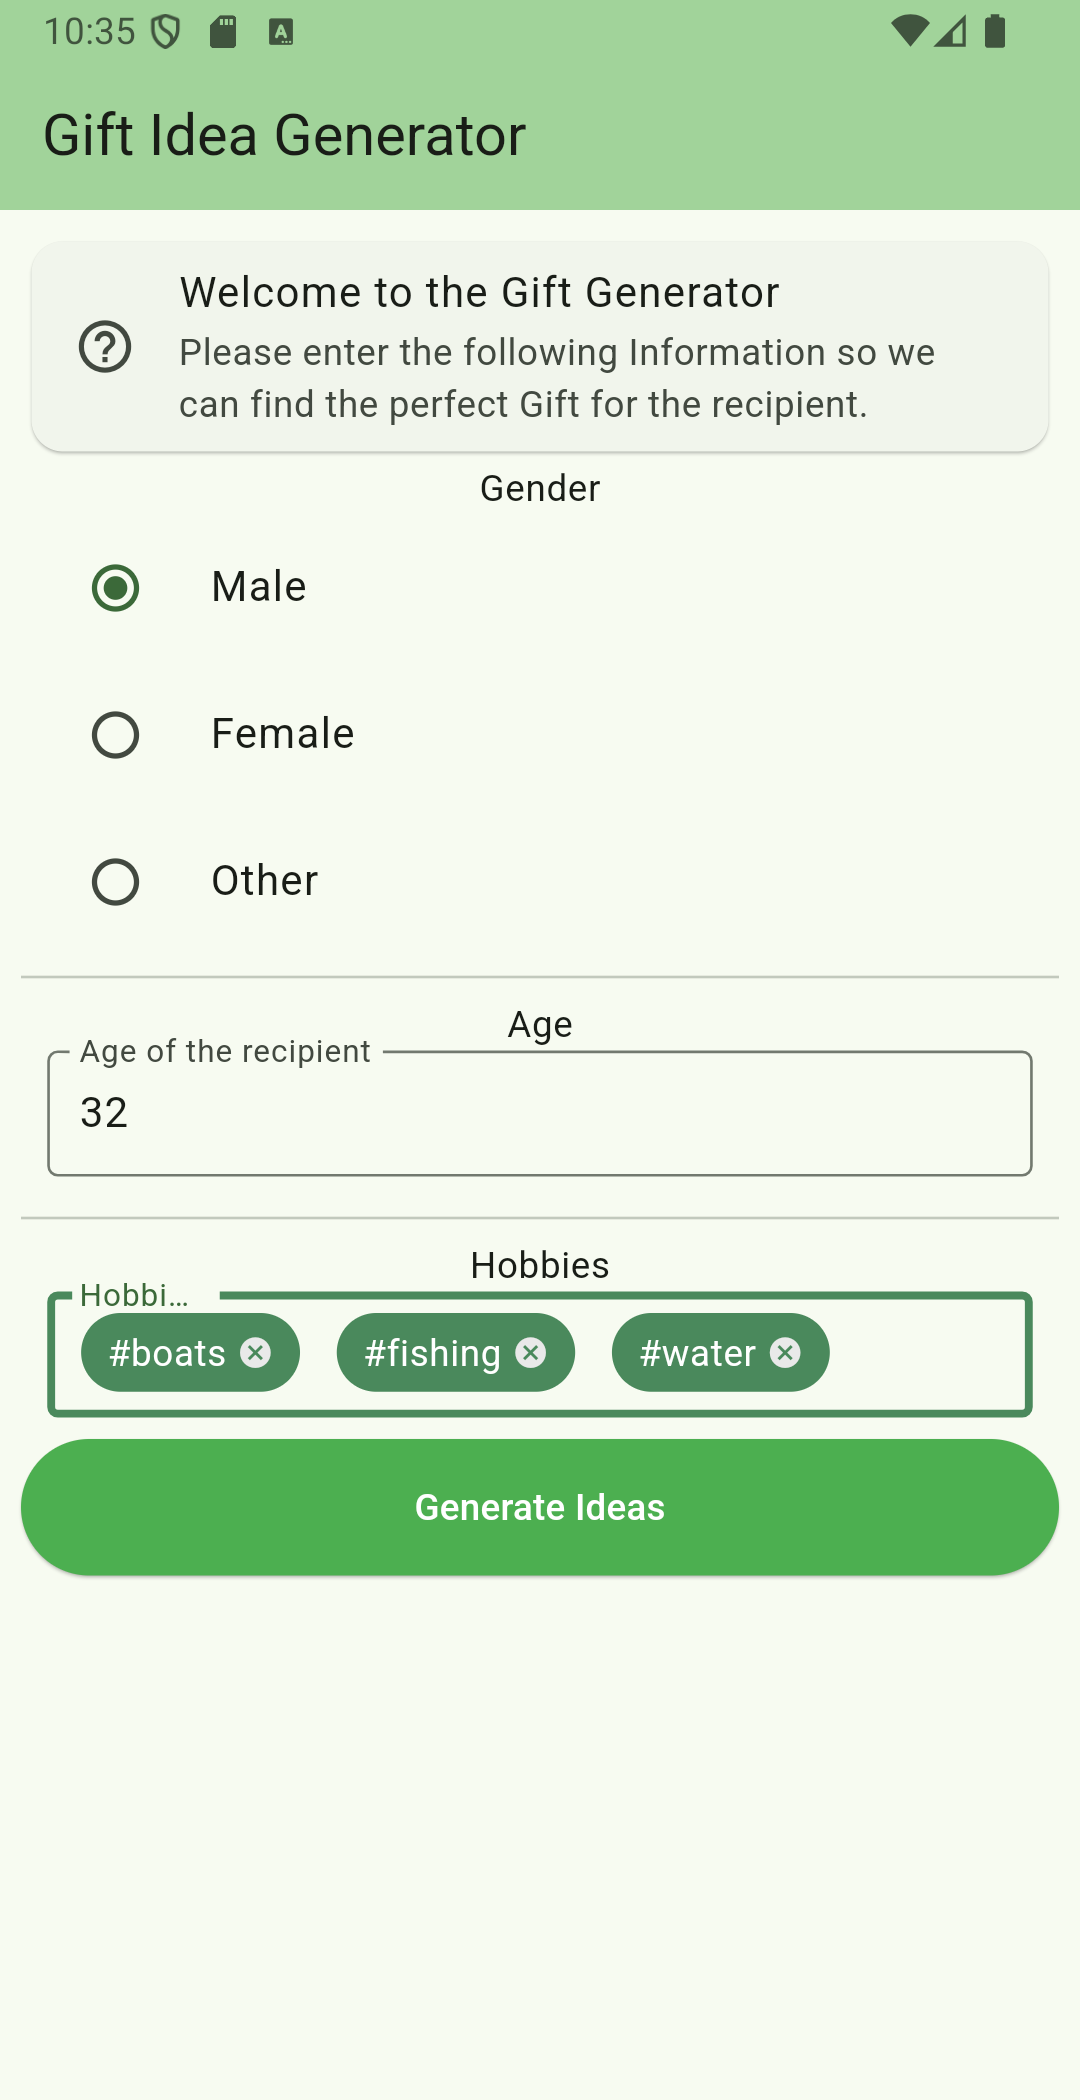
\includegraphics[height=7cm]{figures/screenshots/new_details_view_cropped.png}
		\end{center}
		\caption{\texttt{DetailsView}}
	\end{subfigure}
	\begin{subfigure}{0.5\textwidth}
		\begin{center}
			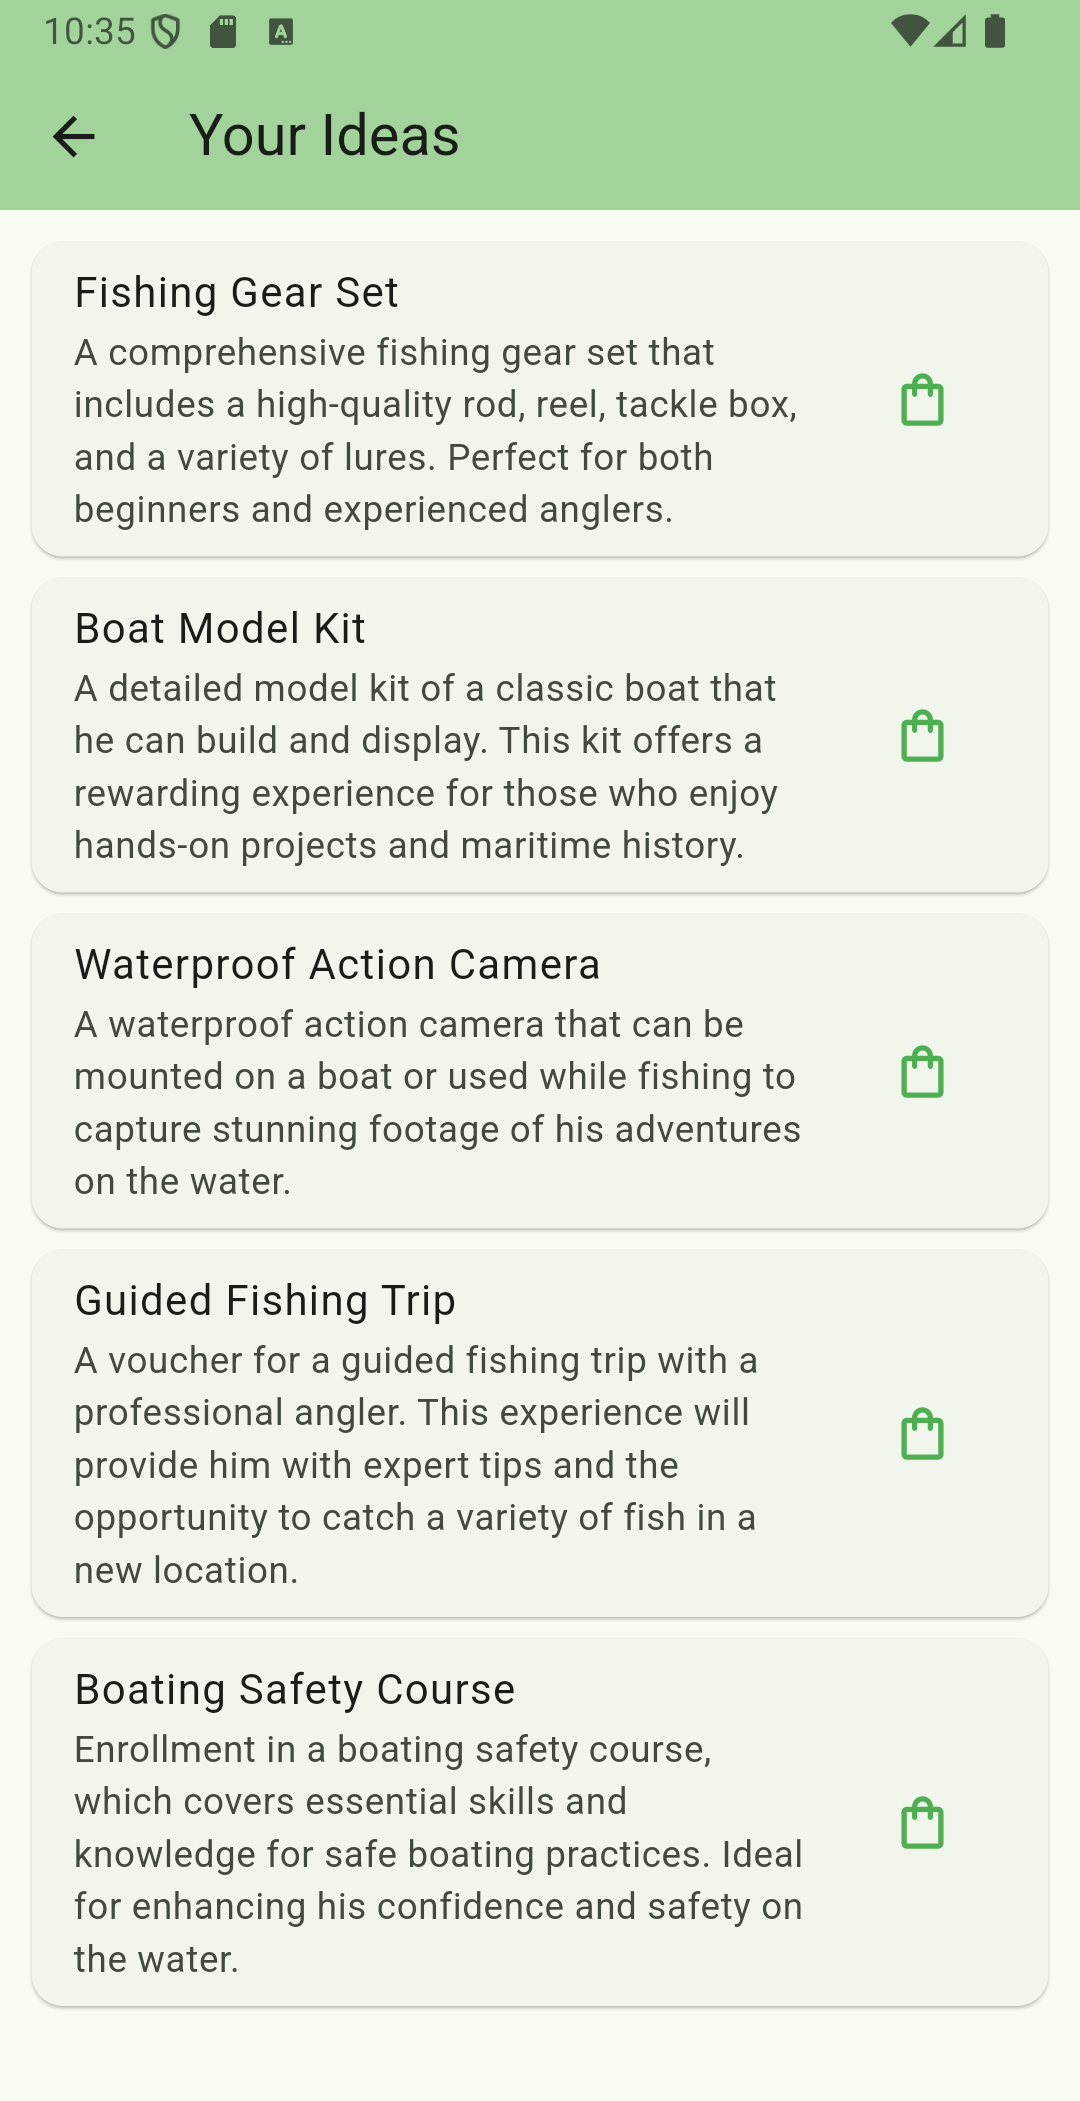
\includegraphics[height=7cm]{figures/screenshots/new_results_view_cropped.png}
		\end{center}
		\caption{\texttt{ResultsView}}
	\end{subfigure}
	\caption{Final Version of the Application}
	\label{fig:finalVersion}
\end{figure}

\section*{OpenAI API Manager}

The \texttt{OpenAI API Manager} is the backend logic which allows the Application to communicate with the OpenAI Assistant. It provides the functionality to convert User Input into a usable text prompt, as well as convert the received JSON into a user-friendly interface.

\begin{figure}[!h]
	\begin{lstlisting}[language=Java]
    // Extracts Gift Ideas from JSON into Idea() Object
    factory GiftResponse.fromJson(Map<String, dynamic> data) {
        GiftResponse gr = GiftResponse();
        for (Map<String, dynamic> idea in data['presents']) { // Extract "present" objects
          gr.ideas.add(Idea(idea["title"], idea['description'])); // Fill information into new Idea() Object
        }
        return gr; // Return a GiftResponse() Object containing Ideas()
    }

    // Takes a Set of Ideas and returns usable Flutter widgets to display in the app
    List<Widget> cards(Set<Idea> ideas) {
        List<Widget> cards = List.empty(growable: true);
        for (Idea idea in ideas) { // For all Ideas in the List
            cards.add(Card( // Add a new widget (Flutter Card Widget in this Case)
            child: ListTile(
                title: Text(idea.title), // Title
                subtitle: Text(idea.description), // Description
                trailing: IconButton( // Shopping Bag Button
                    onPressed: () {
                        _launchUrl(
                            "https://www.galaxus.ch/de/search?searchSectors=0&q=${idea.title}");
                    },
                    icon: Icon(Icons.shopping_bag_outlined, color: Colors.green,))),
            ));
        }
        return cards;
    }
\end{lstlisting}
	\caption{Code section responsible for converting JSON into Widgets}
\end{figure}

%\input{mainmatter/chapter-4} % Create file to add

\chapter{Conclusion}
\label{chapter:conclusion}

\emph{A conclusion...}


%% Prevent urls running into margins in bibliography
\setcounter{biburlnumpenalty}{7000}
\setcounter{biburllcpenalty}{7000}
\setcounter{biburlucpenalty}{7000}

%% Add bibliography
\printbibliography[heading=bibintoc,title=References]

%% ----------------------------------------------------------------------
%%    Appendix (Letters for chapters)
%% ----------------------------------------------------------------------

\appendix

\chapter{Source Code Appendix}
%\label{chapter:title}

\colorlet{punct}{red!60!black}
\definecolor{background}{HTML}{EEEEEE}
\definecolor{delim}{RGB}{20,105,176}
\colorlet{numb}{magenta!60!black}

\lstdefinelanguage{json}{
basicstyle=\normalfont\ttfamily,
numbers=left,
numberstyle=\scriptsize,
stepnumber=1,
numbersep=8pt,
showstringspaces=false,
breaklines=true,
frame=lines,
backgroundcolor=\color{background},
literate=
*{0}{{{\color{numb}0}}}{1}
{1}{{{\color{numb}1}}}{1}
{2}{{{\color{numb}2}}}{1}
{3}{{{\color{numb}3}}}{1}
{4}{{{\color{numb}4}}}{1}
{5}{{{\color{numb}5}}}{1}
{6}{{{\color{numb}6}}}{1}
{7}{{{\color{numb}7}}}{1}
{8}{{{\color{numb}8}}}{1}
{9}{{{\color{numb}9}}}{1}
{:}{{{\color{punct}{:}}}}{1}
{,}{{{\color{punct}{,}}}}{1}
{\{}{{{\color{delim}{\{}}}}{1}
{\}}{{{\color{delim}{\}}}}}{1}
{[}{{{\color{delim}{[}}}}{1}
{]}{{{\color{delim}{]}}}}{1},
}
\begin{figure}[!ht]
    \begin{lstlisting}[language=json]
{
    "name": "present_response_schema",
    "strict": true,
    "schema": {
    "properties": {
        "presents": {
            "type": "array",
            "items": {
                "type": "object",
                "properties": {
                    "description": {
                        "type": "string",
                        "description": "A detailed description of the present."
                    }
                },
                "required": [
                "description"
                ],
                "additionalProperties": false
            }
        }
    },
    "additionalProperties": false,
    "required": [
        "presents"
    ],
    "type": "object"
    }
}
    \end{lstlisting}
    \caption{json schema}
    \label{fig:jsonschema}
\end{figure}
\chapter{Task Division Example}
%\label{chapter:title}

\emph{If a task division is required, a simple template can be found below for convenience. Feel free to use, adapt or completely remove.}

\begin{table}[htb]
    \setlength\extrarowheight{4pt}
    \centering
    \caption{Distribution of the workload}
    \label{tab:taskdivision}
    \begin{tabularx}{\textwidth}{lXX}
        \toprule
        & Task & Student Name(s) \\
        \midrule
        & Summary & \\
        Chapter 1 & Introduction &  \\
        Chapter 2 &  & \\
        Chapter 3 &  & \\
        Chapter * &  & \\
        Chapter * & Conclusion &  \\
        \midrule
        & Editors & \\
        & CAD and Figures & \\
        & Document Design and Layout & \\
        \bottomrule
    \end{tabularx}
\end{table}

%\input{appendix/appendix-c} % Create file to add

\end{document}
